\subsubsection{Transparency} \label{section:transparency}

Some of the trust related issues, which are described in \ref{section:analysisthirdparty}, are caused by the mechanisms for data handling and system parameters being hidden from the users. Centralized systems do not typically reveal their code for public viewing. Data logs, parameters, transaction history, etc. can only be retrieved by the developers and system administrators. Thus, there is no possibility for regular users to check if the system is implemented to follow the guidelines, described in the terms of conditions (assuming that the user has some background and knowledge in software development and programming).

\paragraph{Transparency in blockchain} 
Many public blockchains, including Ethereum, which is used to build the decentralized Secure Package system, are transparent by default. This means that the entire blockchain is accessible by anyone. In case of Ethereum, an easy way to access and visualize the blockchain architecture behind it is to use a block explorer application, such as Etherscan \citep{etherscan}. All of the information about blocks, addresses/accounts (including smart contracts) and transactions is completely transparent and is viewable by using such a service.

\begin{figure}[H]
\centering
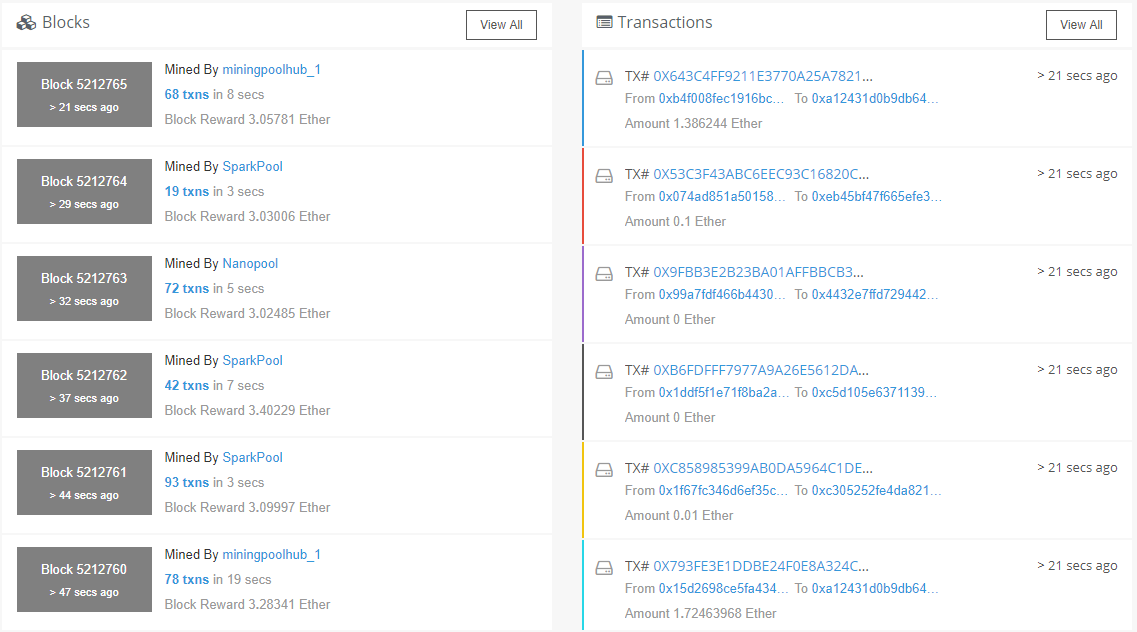
\includegraphics[scale=0.55]{images/etherscan.png}
\caption{Etherscan dashboard, showing recent blocks and transactions.}
\label{fig:etherscanrecent}
\end{figure}

As all of the transaction history is available, it is possible to see the amount of ETH that a given address/account is holding at the moment. Smart contract payload data and their corresponding source code can be viewed as well. In Ethereum, nothing is secret or hidden by default. This complete transparency results in numerous advantages, as well as a number of drawbacks, which are discussed later in this section.

\paragraph{Open source code management} 
Public blockchains are typically categorized as open source type of software. Unlike "closed source", or "proprietary" software, which is managed and controlled only by the person, team, or organization who created it (issues with that are briefly discussed in \ref{section:analysisthirdparty}), the source code of open source software can be inspected, modified, and enhanced by anyone that wishes to do so. In many cases, open source software is more desirable to use, as it typically gives more control to the users, can be used for training and learning, is more secure and is regularly tested by the community, which makes it more stable \citep{opensourceadvantages}.

Everything in Ethereum, including the website, tools, whitepapers and all of the software and compilers are 100\%, open source and is licensed under the GNU General Public License (GPL) \citep{gpl}. The code is constantly developed by the community, that dedicates resources and supports the project by contributing code to Ethereum's public repository \citep{ethereumrepo}. This makes the source code easily modifiable, very secure and thoroughly tested by the community and its administrators.

However, there is also a potential drawback, associated with open-source systems. There have been a few cases, when the bugs that were found in blockchain-based systems were exploited instead of being reported to the developers and fixed. Back in June 2016, the famous DAO hack was performed, by performing the recursive call exploit on the DAO token smart contract. A total of 3.6 million ETH was drained by the attacker within the first few hours of the attack. The aftermath of the DAO hack resulted in a lot of controversy within the Ethereum community \citep{dao}.

\paragraph{Issues with total transparency}
As mentioned before, all of the information, which is relevant to the network, is publicly accessible in Ethereum. This makes the network more trustworthy, as the information flow and transaction history, among other things, can be observed in detail. However, in some cases, like the one which is relevant for this study, namely the implementation of the Secure Package system, this results in some serious privacy-related issues. 

In order for the system to work, personal user data, such as names, addresses, contents of the package, recent GPS location of the package and other sensitive information needs to be stored in the smart contract and processed by the blockchain. There is no built-in data protection mechanisms in the network, thus making all of the personal data visible to the public. This is not desirable at all in context of Secure Package system, as without proper protection against the outsiders, this sensitive information may be used for identity frauds, as described in \ref{section:analysisthirdparty}.


